\section{Detalles de Implementaci'on}
\todomm{intro}
\subsection{Extensi'on de las traducciones Rho}

\todomm{El punto fuerte de tu trabajo fue la implementación de estos conceptos, así que tenemos que explicar bien esto como para que los jurados lo entiendan así. En principio, deberías explicar un poco cómo estaba diseñado Heterogenius, para que se entienda la magnitud del cambio que realizaste}

Debido a los cambios introducidos fue necesario \textit{refactorizar} el diseño de la infraestructura de las traducciones $\rho$. Lo primero que se hizo fue agregar un \textit{TranslationsManager}, un objeto encargado de manejar todas las traducciones soportadas por el sistema. 

Por otro lado los traductores (subclases de \textit{Translator}) deben implementar los tres m'etodos  abstractos definidos en la clase padre. Cada uno de 'estos m'etodos permite un control m'as fino de las traducciones al separar el secuente en sus partes, que son: una referencia de skolemizac'ion, una especificaci'on y la f'ormula analizada.

\begin{figure}[H]
	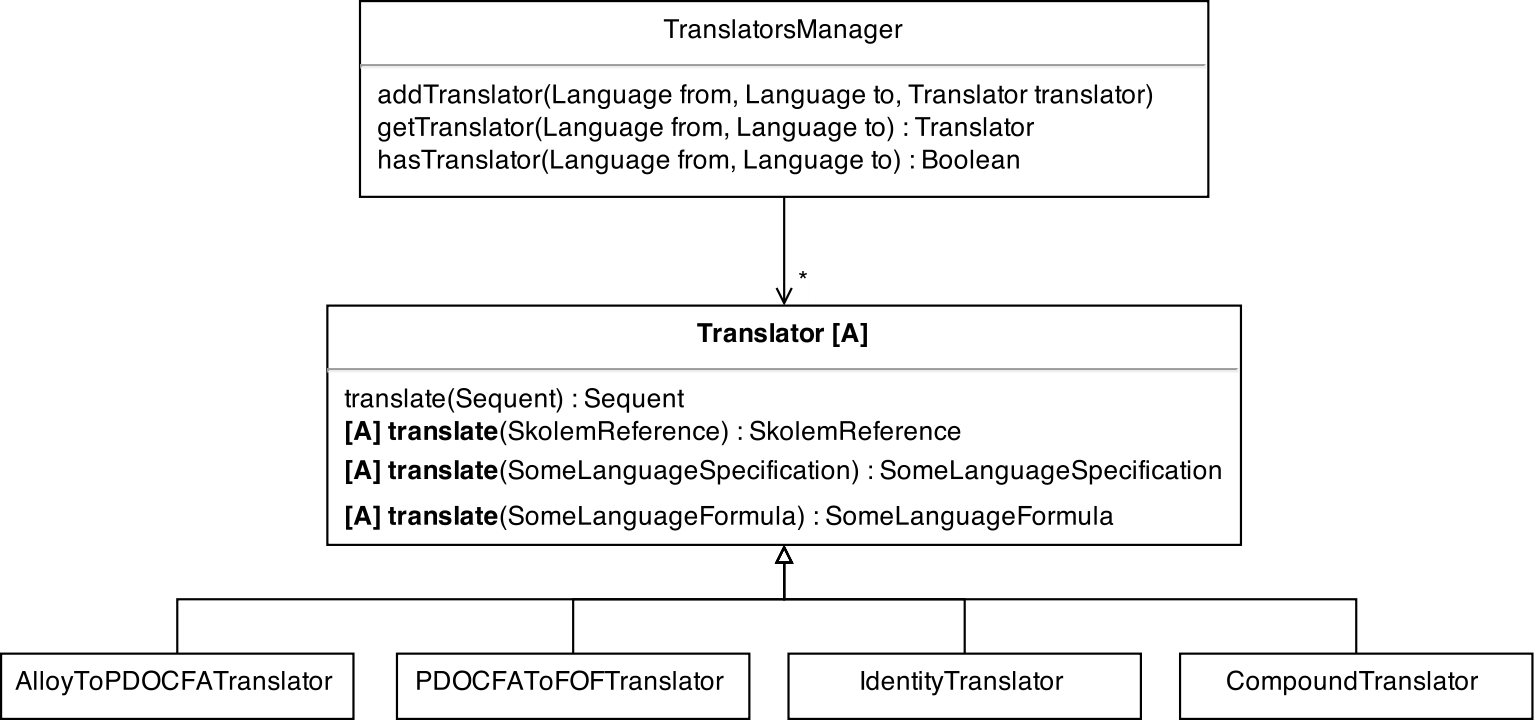
\includegraphics[width=400px, angle=90]{img/arq_traductores.png}
\end{figure}

Se proveen los traductores de \textit{Alloy} a \textit{PDOCFA}, de \textit{PDOCFA} a \textit{TPTP-FOF} asi como el \textit{CompoundTranslator} que permite componer los traductores para lograr traducciones transitivas, por ejemplo de \textit{Alloy} a \textit{TPTP-FOF}.


\subsection{Demostradores de teoremas}

\subsubsection{Preparaci'on del secuente}

El formato \textit{TPTP-FOF} que usan las herramientas autom'aticas agregadas es una lista de f'ormulas escritas en el lenguaje \textit{TPTP-FOF}. Cada una de 'estas f'ormulas debe tener un tipo que puede ser: \textit{axiom} o \textit{conjecture} (existen m'as tipos pero son irrelevantes para nuestro caso).

Para convertir el secuente analizado al formato \textit{TPTP-FOF} se agregan todas las f'ormulas del antecedente con el tipo \textit{axiom} y las f'ormulas del consecuente con el tipo \textit{conjecture}. 

Al ejecutar un demostrador autom'atico con la entrada preparada de este modo, se va a tratar de probar las f'ormulas del consecuente usando que las f'ormulas del antecedente son verdaderas.


\subsubsection{Integraci'on con Heterogenius}

Para integrar las herramientas autom'aticas, tanto los demostradores de teoremas como los buscadores de contraejemplos fue necesario \textit{refactorizar} y extender el diseño de algunas partes de la arquitectura de Heterogenius. Algunos de los objetivos y criterios que se usaron durante el rediseño fueron lograr abstraer las herramientas usadas y hacer un diseño lo suficientemente extensible y abierto para la integraci'on con nuevas herramientas en el futuro.

\begin{figure}[H]
	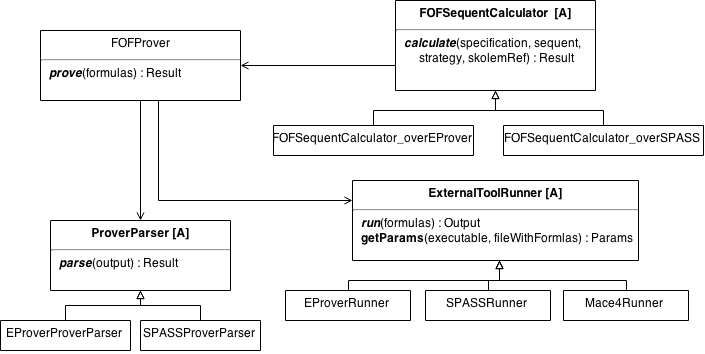
\includegraphics[width=450px, angle=90]{img/arq_prover.png}
	\centering
	\caption{Demostradores autom'aticos usados como calculadores de secuentes.}
\end{figure}

\todomm{Mencionar en la explicación qué roles desempeñan cada una de las entidades mencionadas. Además indicar explícitamente cuáles debieron ser modificadas y cuáles agregadas en la nueva versión.
Para explicar esto podés indicar los pasos que se deberían seguir para incorporar un demostrador nuevo (como lo que está en estos dos párrafos, pero explicado con más detalle).
Y explicar cómo fueron implementados esos pasos para incluir alguno de los demostradores que agregaste.}

Un calculador de secuentes basado en un demostrador autom'atico del lenguaje \textit{TPTP-FOF} se crea subclasificando la clase abstracta \textbf{FOFSequentCalculator}. La nueva clase va a contener un objeto \textit{FOFProver} compuesto con los objetos de las subclases de \textbf{ProverParser} y de \textbf{ExternalToolRunner} correspondientes.

Para agregar una herramienta nueva primero se debe subclasificar la clase abstracta \textbf{ExternalToolRunner}. Esta clase abstrae las particularidades de ejecuci'on de la herramienta especificando los parametros necesarios. Luego se extiende la clase \textbf{ProverParser} que se encarga de procesar el texto correspondiente a la salida de la herramienta. 



\subsection{B'usqueda de contraejemplos}

\subsubsection{Preparaci'on del secuente}

Tanto \textit{Mace4} como \textit{E-Prover} se usan para buscar contraejemplos de los secuentes \textit{TPTP-FOF}. Como las dos herramientas son buscadores de modelos, para preparar el secuente lo que se hace es armar una lista de f'ormulas de tipo \textit{axiom} a partir de las f'ormulas del antecedente y del consecuente del secuente analizado.

Cuando todas las f'ormulas que se envian como entrada a los buscadores de modelos son de tipo \textit{axiom}. Las herramientas tratan de buscar un modelo para el conjunto de los axiomas recibidos.

Lo que se quiere lograr es encontrar un contraejemplo, entonces se hace necesario negar el secuente y buscar un modelo para la negaci'on.

Sea $\{\alpha_1 \dots \alpha_n\} \vdash \{\beta_1 \dots \beta_m\}$ el secuente bajo an'alisis.
La negaci'on se puede escribir como:

\begin{equation}
\bigwedge\limits_{i=1}^n{\alpha_i} \wedge \bigwedge\limits_{j=1}^m{\neg \beta_{j}}
\end{equation}

Con lo cual para armar la lista de f'ormulas de entrada, para cada $\alpha_{i}$ del antecedente se agrega $\alpha_{i}$ como axioma y para cada $\beta_{i}$ del consecuente se agrega $\neg \beta_{i}$ tambi'en como axioma.

Encontrar un modelo para una especificaci'on armada de 'este modo implica la existencia de un contraejemplo para el secuente procesado.


\subsubsection{Integraci'on con Heterogenius}

Tambi'en como en el caso de los demostradores autom'aticos fue necesario \textit{refactorizar} el diseño de los buscadores de contraejemplos para permitir una mayor flexibilidad a la hora de agregar nuevas herramientas con soporte de \textit{TPTP-FOF}.

\begin{figure}[H]
	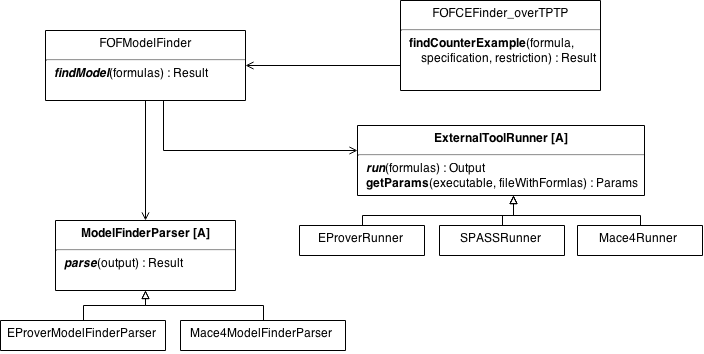
\includegraphics[width=450px, angle=90]{img/arq_ce.png}
	\centering
	\caption{Buscadores de contraejemplos.}
\end{figure}

\todomm{Ídem anterior (a menos que queden demasiado parecidos).}
El diseño de los buscadores de contraejemplos basados en \textit{TPTP-FOF} es an'alogo a los calculadores de secuentes. Se usa la misma clase \textbf{ExternalToolRunner} que en el caso anterior para la abstracci'on de la ejecuci'on de la herramienta en s'i. Pero en lugar de subclasificar \textbf{ProverParser} se subclasifica la clase abstracta \textbf{ModelFinderParser} que tiene un comportamiento an'alogo.